\section{Faster Regional-CNN}

\subsection{Stage 1: Region Proposal Network (RPN)}
In the first stage, a Convolutional Neural Network (CNN) is used to extract a feature map from the input image. Each pixel in the feature map is treated as an anchor point, and multiple anchor boxes are associated with each anchor point. These anchor boxes are compared with the ground truth bounding boxes of objects in the image. If the Intersection over Union (IoU) score of an anchor box with a ground truth box is greater than a certain threshold (e.g., 0.7), it is considered a positive box. The anchor box with the highest IoU score is selected.

For each positive anchor box, a corresponding ground truth box is derived. These boxes are then filtered based on the positive boxes (red). Since each ground truth box is associated with a specific category (e.g., car, person), we can apply the same principle to obtain positive categories.

Next, the offsets of the anchor boxes to the ground truth boxes are calculated. This information is used to adjust the anchor boxes and generate region proposals, which are potential object bounding boxes that are likely to contain objects of interest (Anchor Box + Offset = Region Proposal).

CNN Backbone extracts a feature map. Each pixel of the feature map becomes an anchor point. There are 9 different anchor boxes (feature map* 9). Each \textbf{anchor box} is compared with the ground truth box. If the score \textgreater{} 0.7, it is a positive box. The highest score wins. To compare IoU is used.
For each anchor box, we derive a corresponding ground truth box and filter them based on positive boxes (red). Since each ground truth box has a category, we can apply the same principle to obtain positive categories. Next, we calculate the offsets of the anchor boxes to the ground truth boxes. Fig \ref{fig:faster_r_cnn_stage_1}

\begin{figure}[ht]
  \centering
  \subfloat[IoU]{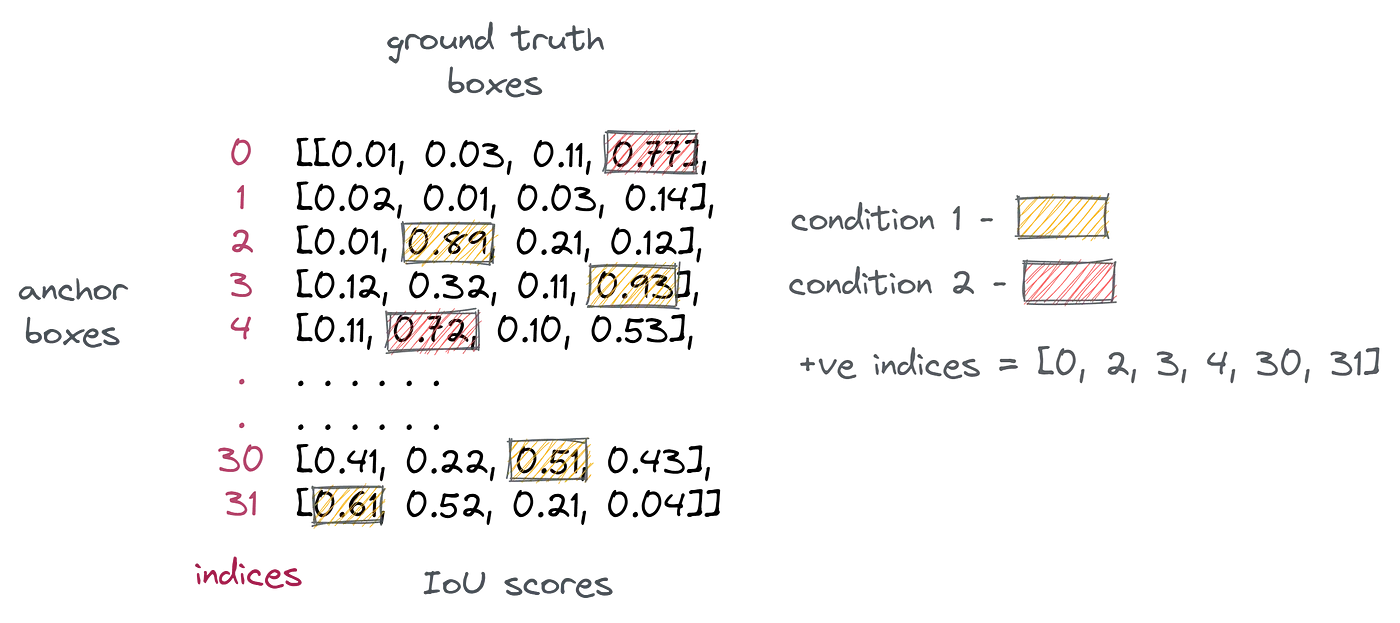
\includegraphics[width=0.5\textwidth]{images/faster_r_cnn/positive_anchor.png}\label{fig:f1}}
  \hfill
  \subfloat[Filter Positive Groundtruth]{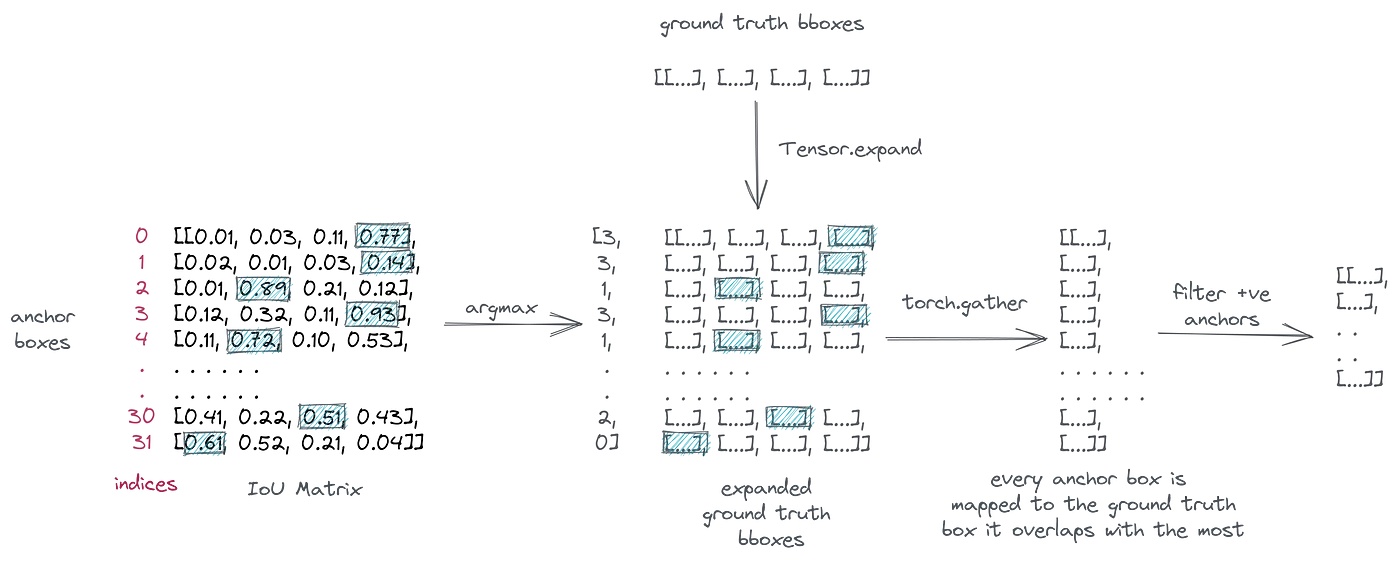
\includegraphics[width=0.5\textwidth]{images/faster_r_cnn/filter_positive_gt.png}\label{fig:f2}}
  \caption{Stage 1: Region Proposal Network (RPN)}
  \label{fig:faster_r_cnn_stage_1}
\end{figure}

\subsection{Stage 2: ROI Pooling and Prediction}
In the second stage, the region proposals are divided into a fixed number of regions and max pooling is applied to each region. This operation, known as Region of Interest (ROI) pooling, ensures that the regions have the same dimension regardless of the size of the original region proposal. This is important because it allows the network to use fully connected layers to make predictions.

After ROI pooling, the regions are passed through a series of fully connected layers to make predictions. Two types of predictions are made for each region: a class prediction (using softmax) and a bounding box prediction. The class prediction is made using a cross-entropy loss function, and the bounding box prediction is made using a regression loss function.

The final output of the Faster R-CNN algorithm is a set of bounding boxes and associated class labels for the objects detected in the image.
Fig \ref{fig:faster_r_cnn_structure}

\begin{figure}[H]
  \centering
  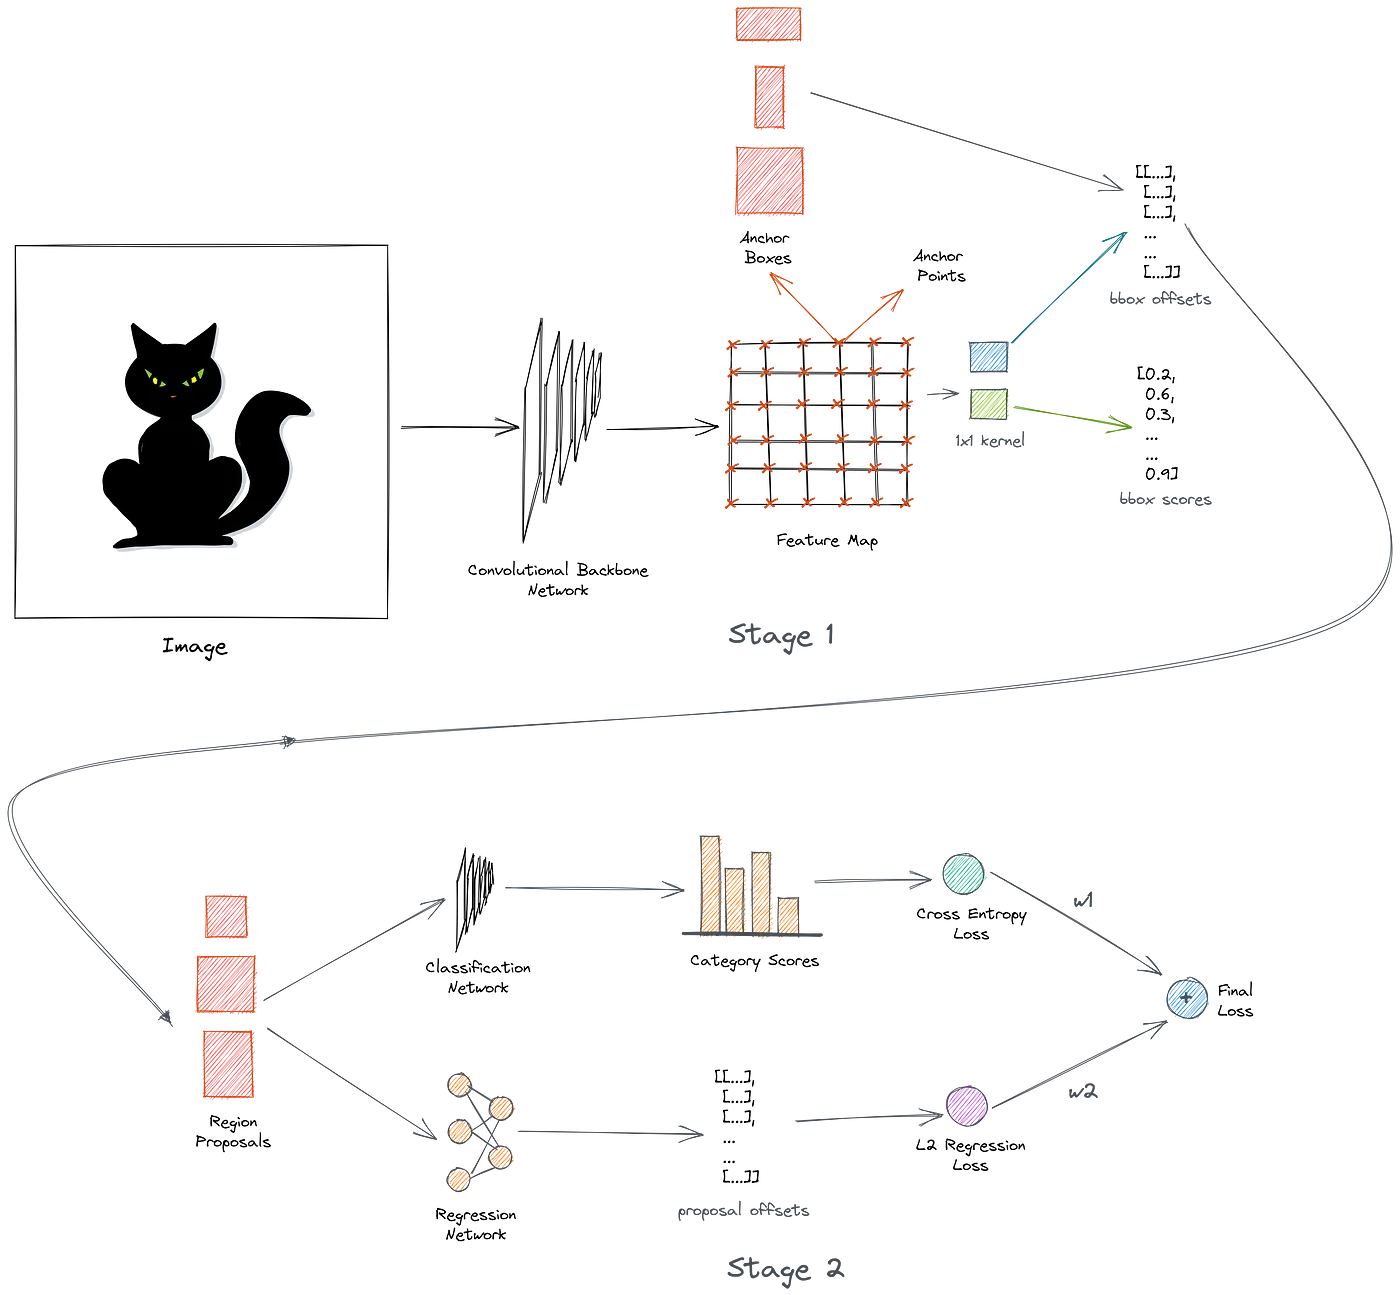
\includegraphics[width=0.5\textwidth]{images/faster_r_cnn/structure.png}
  \caption{Faster RCNN}
  \label{fig:faster_r_cnn_structure}
\end{figure}

\subsection{Sources}

\begin{enumerate}
  \item \href{https://towardsdatascience.com/understanding-and-implementing-faster-r-cnn-a-step-by-step-guide-11acfff216b0}{Understanding and Implementing Faster R-CNN: A Step-By-Step Guide}
\end{enumerate}
